The first layer of the vest is the music player layer. This layer is responsible for connecting the music player to the vest and the vest website. The different subsystems within this layer are the music player, the website, and the Raspberry Pi. The music player system is contingent upon whatever device/player the user prefers. This is a black-box system that will not be designed by the Sound Squad team.

\subsection{Website}
The website will serve as a means of product information/instructions, possible play list creation and management, and point of sale for purchase of other Sound Squad items. The website will communicate with the music player using API calls, and communicate with the vest through a programmed connection with the vest's Raspberry Pi. The website will have a database subsystem for user authentication and saving user settings and playlists.

\begin{figure}[h!]
	\centering
 	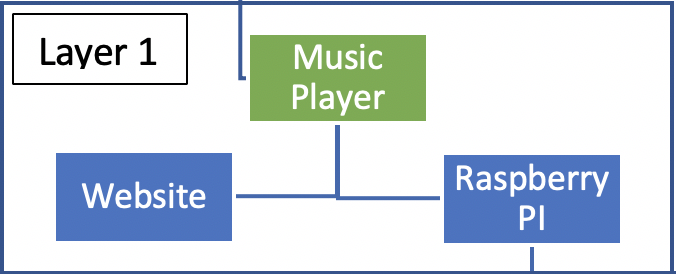
\includegraphics[width=0.60\textwidth]{images/subsystem1}
 \caption{Example subsystem description diagram}
\end{figure}

\subsubsection{Assumptions}
Sound squad has made the assumption that APIs exist for all required functionality and interface between the website and the music player. Sound squad also made the assumption that users will have Wifi for the connection of the website changes to the Raspberry Pi.

\subsubsection{Responsibilities}
The website will be responsible for allowing the user to login to the Sound Squad site and connect to the music player site, make purchases of new products, create playlists and select songs to play, and finally to make advanced settings changes.

\subsubsection{Subsystem Interfaces}
The website will make an API call out to the music player and receive a rest endpoint containing the request/data. The website will connect to a Raspberry Pi via WiFi.

\begin {table}[H]
\caption {Subsystem interfaces} 
\begin{center}
    \begin{tabular}{ | p{1cm} | p{6cm} | p{3cm} | p{3cm} |}
    \hline
    ID & Description & Inputs & Outputs \\ \hline
    \#1 & Connection to the music player & \pbox{3cm}{API call} & \pbox{3cm}{API endpoint}  \\ \hline
    \#2 & Connection to the Raspberry Pi & \pbox{3cm}{NA} & \pbox{3cm}{Music signal}  \\ \hline
    \end{tabular}
\end{center}
\end{table}

\subsection{Raspberry Pi}
This section should be a general description of a particular subsystem for the given layer. For most subsystems, an extract of the architectural block diagram with data flows is useful. This should consist of the subsystem being described and those subsystems with which it communicates.

\begin{figure}[h!]
	\centering
 	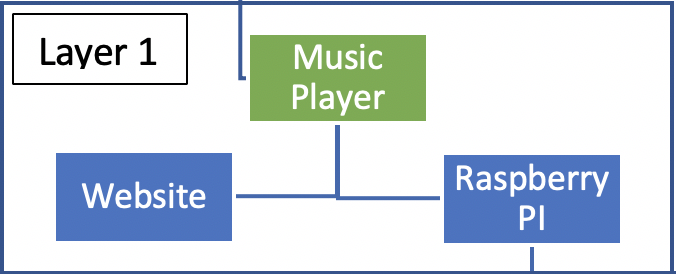
\includegraphics[width=0.60\textwidth]{images/subsystem1}
 \caption{Example subsystem description diagram}
\end{figure}

\subsubsection{Assumptions}
Any assumptions made in the definition of the subsystem should be listed and described. Pay particular attention to assumptions concerning interfaces and interactions with other layers.

\subsubsection{Responsibilities}
Each of the responsibilities/features/functions/services of the subsystem as identified in the architectural summary must be expanded to more detailed responsibilities. These responsibilities form the basis for the identification of the finer-grained responsibilities of the layer's internal subsystems. Clearly describe what each subsystem does.

\subsubsection{Subsystem Interfaces}
Each of the inputs and outputs for the subsystem are defined here. Create a table with an entry for each labelled interface that connects to this subsystem. For each entry, describe any incoming and outgoing data elements will pass through this interface.

\begin {table}[H]
\caption {Subsystem interfaces} 
\begin{center}
    \begin{tabular}{ | p{1cm} | p{6cm} | p{3cm} | p{3cm} |}
    \hline
    ID & Description & Inputs & Outputs \\ \hline
    \#xx & Description of the interface/bus & \pbox{3cm}{input 1 \\ input 2} & \pbox{3cm}{output 1}  \\ \hline
    \#xx & Description of the interface/bus & \pbox{3cm}{N/A} & \pbox{3cm}{output 1}  \\ \hline
    \end{tabular}
\end{center}
\end{table}



